\documentclass[11pt,letterpaper]{article}
\usepackage[margin=0.7in]{geometry}
\usepackage[T1]{fontenc}
\usepackage{lmodern,microtype,graphicx,booktabs,amsmath,xcolor,fancyhdr,array}
\usepackage[hidelinks]{hyperref}
\usepackage[font=small,labelfont=bf]{caption}
\setlength{\parindent}{0pt}\setlength{\parskip}{7pt}\setlength{\emergencystretch}{4em}
\pagestyle{fancy}\fancyhf{}\fancyhead[L]{Manufacturing energy exposure}
\fancyhead[R]{Independent research manuscript}
\fancyfoot[L]{29 October 2026 --- not peer reviewed}\fancyfoot[R]{\thepage}
\setlength{\headheight}{14pt}
\begin{document}
{\LARGE\bfseries Output prices change the explanation\\of manufacturing energy use\par}
\vspace{8pt}
{\large A matched-price accounting comparison in four euro-area countries\par}
{\small James N. Jean IV \quad Independent, AI-assisted research example \quad 29 October 2026\par}
\section*{Executive summary}
An analyst screening industrial energy exposure needs to distinguish production scale, industry mix and energy use per unit of output. A current-price output denominator mixes output volume with prices. Using Eurostat physical energy and gross-output accounts for 2015--2023, this study compares the same established additive decomposition under current-price and matched previous-year-price output.

Germany's linked 2019--2023 intensity contribution is $-1{,}524.4$ PJ using current prices and $-420.6$ PJ using matched prices, while its observed energy-use change is $-622.5$ PJ under either calculation. The denominator changes the accounting explanation, not the physical total. All four countries have a less negative intensity contribution under matched prices in this period.

\begin{center}\small
\begin{tabular}{lrrr}\toprule
Country & Observed energy change & Current-price intensity & Matched-price intensity\\
 & PJ & PJ & PJ\\\midrule
Belgium & -156.4 & -344.3 & -32.3\\
Germany & -622.5 & -1,524.4 & -420.6\\
France & -304.4 & -594.3 & -169.2\\
Netherlands & -140.4 & -492.5 & -107.0\\\bottomrule
\end{tabular}
\captionof{table}{Linked annual contributions over 2019--2023. Intensity is one component of an exact activity--structure--intensity identity; it is not the whole observed change or a causal savings estimate. PJ = 1,000 TJ.}
\end{center}

Across 608 annual country--industry transitions, 82 (13.5\%) have opposite signs of intensity change under the two price bases. Yet the five highest-intensity industry sets in 2023 are unchanged in every country. Price sensitivity matters for interpreting trends; it need not overturn a broad high-exposure screen.

Use matched-price annual output alongside physical energy totals when discussing intensity progress, and retain a nominal comparator to expose denominator sensitivity. Before judging a particular plant or investment, obtain process-level output, energy prices, product mix and operating conditions. These aggregate accounts cannot establish engineering efficiency, energy-bill inflation, causality, carbon impacts or realized financial returns.

The eligible panel contains Belgium, Germany, France and the Netherlands. Spain and Italy fail the fixed source gate; together they represent 28.9\% of 2023 manufacturing energy in the original six-country candidate set. Germany retains provisional source flags. These are current historical revisions, not real-time information vintages. The contribution is a reproducible, bounded comparison and its stable-ranking counterpoint, not a new decomposition method or a claim to comprehensive European coverage.

\newpage
\section*{1. Sources, population and measurement}
The fixed candidate countries were Belgium, Germany, Spain, France, Italy and the Netherlands, all using the euro. Years were 2015--2023. Nineteen mutually exclusive NACE Rev.2 manufacturing groups were fixed before full retrieval. The published aggregate C is a reconciliation target; it is never added to its constituent industries.

Eurostat \texttt{env\_ac\_pefa04} supplies annual net domestic energy use, indicator \texttt{NETDOM\_EUSE}, in TJ [1]. This account includes energy and non-energy uses and follows the source's residence/accounting boundary. It is not final fuel consumption, an energy footprint or a firm-level measure. Eurostat \texttt{nama\_10\_a64}, item P1, supplies gross output in million euro at current prices (CP) and previous-year prices (PYP), with official \texttt{CLV\_I15} volume indices for a separate check [2]. Gross output includes intermediate production transactions; it is not GDP or value added.

Twelve sequential API responses were retained on 29 October 2026, with exact compressed bytes, original-response hashes, request filters, update labels and retrieval timestamps [3]. The snapshot contains 4,320 selected cells, including missing values, and 1,080 normalized country--year--group records, including C. Statistics and metadata are reused with Eurostat attribution and a modification notice [4]. No source paper, private record or individual data is redistributed.

Eligibility requires positive, finite energy, CP and PYP values for every group and year. Nineteen-group sums must reconcile to C within 2 TJ or 2 million euro, as applicable. Break/definition flags b/d exclude the affected country. At least four complete countries are required. Spain lacks all 180 required PYP cells, including C; Italy has the same missingness and a published break flag. Neither is imputed. Belgium, Germany, France and the Netherlands pass unchanged criteria. Their source-aggregate discrepancies are at most 0.3 source units. German provisional flags remain visible.

\section*{2. Established accounting method}
For an annual transition, let $E_{i0},E_{i1}>0$ be industry energy use. In the matched-price calculation, $q_{i0}$ is prior-year CP output and $q_{i1}$ is current-year PYP output. They share the prior year's prices. Define $A_t=\sum_i q_{it}$, $s_{it}=q_{it}/A_t$ and $I_{it}=E_{it}/q_{it}$. The identity $E_t=\sum_i A_ts_{it}I_{it}$ gives additive LMDI contributions [5,6]:
\[
 D_A=\sum_i L_i\log\frac{A_1}{A_0},\qquad
 D_s=\sum_i L_i\log\frac{s_{i1}}{s_{i0}},\qquad
 D_I=\sum_i L_i\log\frac{I_{i1}}{I_{i0}},
\]
where $L_i=(E_{i1}-E_{i0})/(\log E_{i1}-\log E_{i0})$ and $L_i=E_{i0}$ for equal endpoints. Then $D_A+D_s+D_I=E_1-E_0$. The nominal comparator uses current-year CP output instead of PYP, retaining the same energy observations.

Annual effects are added over 2015--2023 and 2019--2023. The linked sums reconcile to endpoint energy changes in TJ. PYP levels are not a homogeneous price-base time series; annual matched prices support this calculation. Chained industry volume indices are checked individually and never summed, because chain-linked component levels are generally non-additive [2]. There is no fitted model, tuning or claim that the intensity term isolates technical efficiency.

\newpage
\section*{3. Attribution changes; physical energy does not}
\begin{center}
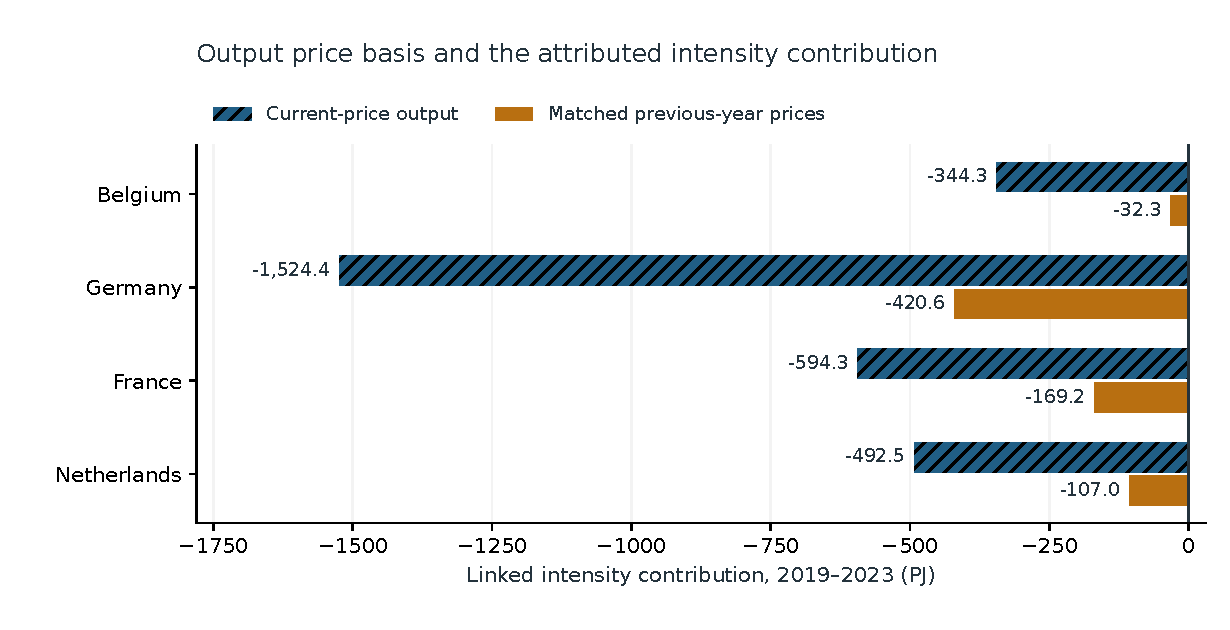
\includegraphics[width=\linewidth]{images/intensity_contributions.pdf}
\captionof{figure}{Same observations, different output denominators. Bars show the linked intensity component, not total energy use. Both full decompositions reconcile to the same physical change. Source: retained Eurostat accounts; original calculations.}
\end{center}

For Germany in 2019--2023, matched-price activity, structure and intensity contributions are $-20.9$, $-181.1$ and $-420.6$ PJ. The nominal calculation instead attributes $+770.1$ PJ to activity, $+131.8$ PJ to structure and $-1{,}524.4$ PJ to intensity. Each sums, before display rounding, to the same $-622.5$ PJ change. This reallocation is an accounting consequence of the chosen denominator, not an experiment that identifies a price shock.

The longer 2015--2023 window also cautions against a simple efficiency narrative. Belgium's current-price intensity contribution is $-326.2$ PJ; its matched-price contribution is $+74.1$ PJ, although physical energy falls by $98.3$ PJ. Changes in production composition and other unobserved conditions still enter these aggregate terms.

\begin{center}\small
\begin{tabular}{lrr}\toprule
Country & All-industry matched intensity & Omit-one-industry range\\
 & PJ, 2019--2023 & PJ, 2019--2023\\\midrule
Belgium & -32.3 & [-50.3, -6.7]\\
Germany & -420.6 & [-431.8, -152.7]\\
France & -169.2 & [-173.6, -97.3]\\
Netherlands & -107.0 & [-110.1, -56.7]\\\bottomrule
\end{tabular}
\captionof{table}{Each of nineteen sensitivity runs removes one industry and recomputes each annual decomposition, including output totals and shares, before linking. Ranges describe accounting sensitivity; they are not confidence intervals. The aggregate decline in this component remains negative under every omission.}
\end{center}

The full package retains 64 annual country--basis decompositions, 16 linked country--window--basis results and 1,216 annual omit-one-industry decompositions. All outcomes, including unfavorable and stable comparisons, are retained.

\newpage
\section*{4. Industry trends can reverse sign}
\begin{center}
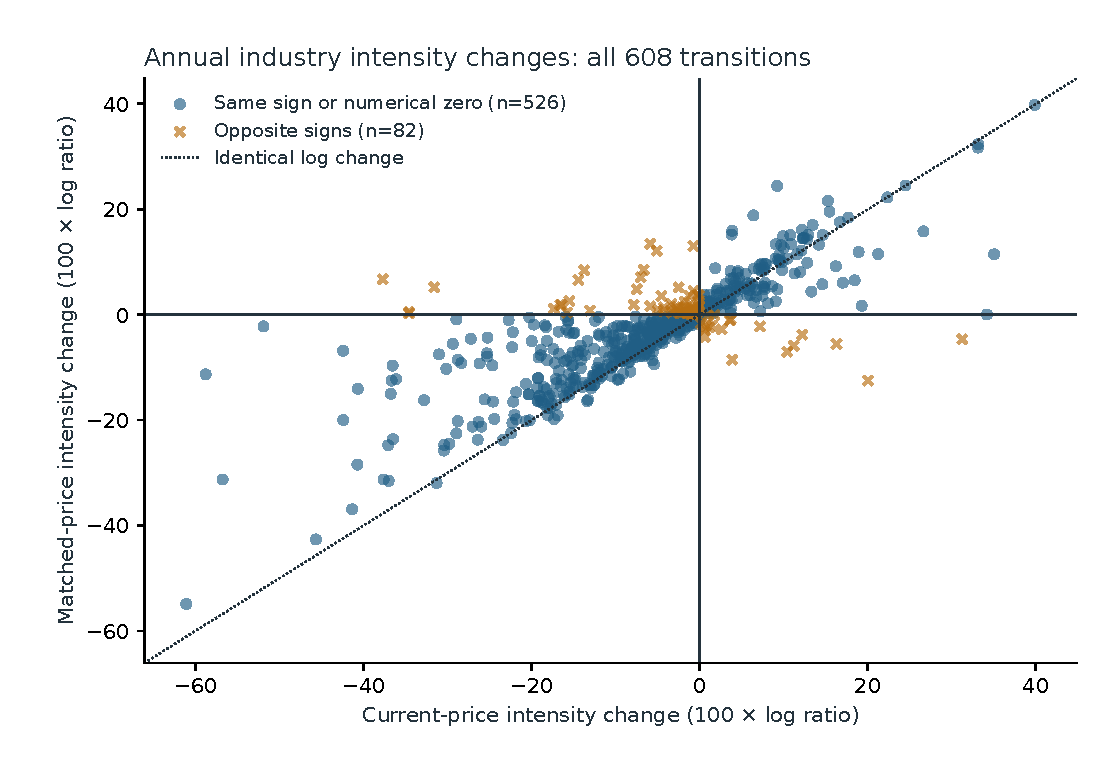
\includegraphics[width=.97\linewidth]{images/industry_contrasts.pdf}
\captionof{figure}{All four countries, nineteen groups and eight annual transitions. Each axis is 100 times a log intensity ratio, not a percentage change. Crosses mark opposite signs exceeding the fixed numerical zero guard. Overlapping marks can hide individual observations; all 608 rows remain available. Source: retained Eurostat accounts; original calculations.}
\end{center}

For an industry, matched-price minus nominal log intensity change equals $\log(\mathrm{CP}_t/\mathrm{PYP}_t)$. This exact wedge is independently reconstructed for every transition. The opposite-sign criterion requires both changes to exceed $10^{-10}$ in absolute log units; this is a numerical zero guard, not a business-materiality cutoff.

Belgium has 22 of 152 opposite-sign transitions, Germany 18 of 152, France 24 of 152 and the Netherlands 18 of 152. The annual counts across countries are 7, 13, 12, 11, 7, 9, 10 and 13 from 2016 through 2023. Sign reversals occur throughout the window; they are not solely a 2023 result. The figure and counts describe these observed accounts, with no sampling inference.

The 2023 ranking question is different. Ranking energy divided by CP and by PYP produces the same top-five industry set in each country. Full-rank changes occur in 6 of 19 Belgian groups, 2 of 19 German groups, none in France and 2 of 19 Dutch groups. Germany swaps ordering within the top five. Stable top-five membership is a useful counterpoint to price-sensitive trend attribution; it does not establish that rankings are robust to every alternative output definition, year or country.

\newpage
\section*{5. The high-exposure screen remains stable in 2023}
\begin{center}
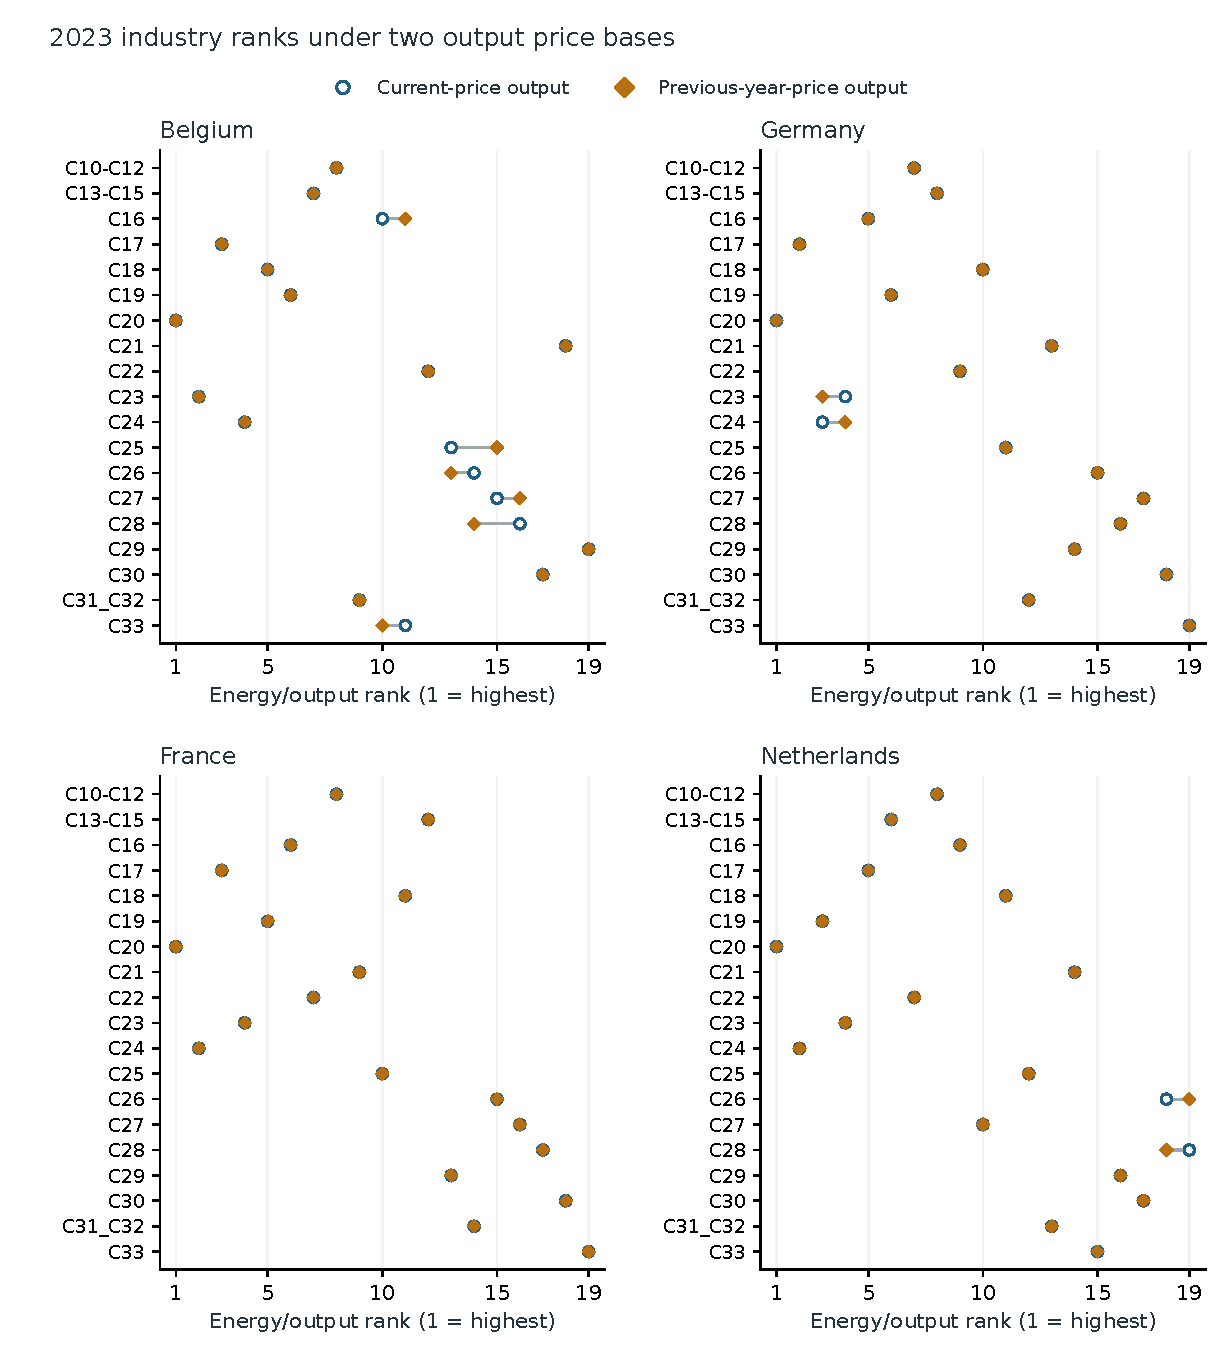
\includegraphics[width=.89\linewidth]{images/industry_rankings.pdf}
\captionof{figure}{All nineteen industry ranks within each country. Rank 1 is the highest energy/output ratio. Open circles use current prices; diamonds use previous-year prices. Connected pairs show ordering differences, not a time transition. Codes and full labels are in the retained panel and Appendix A. Ratios are not suitable for engineering-efficiency league tables across countries.}
\end{center}

\newpage
\section*{6. Independent checks, reproducibility and limits}
The protocol and source accounting were committed before analytic development. Germany, France and the Netherlands supplied development outcomes. The analysis code and eight dependency hashes were frozen and pushed before Belgium's decompositions, intensity contrasts, volume indices and rankings were computed. All six countries' source-coverage energy totals were allowed earlier solely to describe exclusions. Belgium checks implementation transfer; it is not a random population holdout or a forecasting test.

Seven boundary tests cover equal endpoints, activity-only, structure-only, intensity-only, energy-unit scaling, output-unit invariance, ordering and invalid inputs. A separate mixed-radix JSON-stat decoder and SQL path reconstruct all 4,320 cells and eligibility decisions. A separate 50-digit Decimal log-difference implementation imports no main analysis helper and checks every effect, linked endpoint, price wedge, index, rank and omission run: 16,724 numerical comparisons for the four-country analysis.

Scientific comparisons use unchanged absolute $10^{-7}$ and relative $10^{-9}$ tolerances; these differ from source-rounding allowances. The retained maximum decomposition residual is below $1.1\times10^{-9}$ TJ. All 684 reconstructed industry-year indices differ from the official, 2015-rebased volume indices by at most 0.0118 index points, within the 0.25-point source-series bound fixed before index calculation. This checks source consistency and code, not official measurement accuracy. A fresh isolated replay rebuilds 42,515 CSV numerical values from the retained responses without network access.

There are no sampling confidence intervals: these are revised published accounts and a convenience panel, with no microdata sampling model. Source revisions, provisional flags, output/product composition and energy-accounting boundaries remain material uncertainties. The 28.9\% excluded-energy share refers only to the six candidate countries in 2023, not all Europe. No comprehensive literature search or scientific-novelty claim is made. LMDI is established [5,6]; the contribution is the transparent matched-versus-nominal comparison, all source exclusions and its stable-ranking result.

Code, source bytes, all result tables, the frozen protocol and original figures are available in the project repository. Reproduction checks statistical outputs; PDF rendering is checked separately. Release status requires exact-head Linux CI, reviewed-file privacy checks, matching tested/merged trees and a verified annotated tag. This manuscript makes no journal-submission or peer-review claim.

\section*{References}
\small
[1] Eurostat. Physical energy flow accounts metadata and dataset \texttt{env\_ac\_pefa04}. \url{https://doi.org/10.2908/env_ac_pefa04}. Metadata: \url{https://ec.europa.eu/eurostat/cache/metadata/EN/env_pefa_sims.htm}.

[2] Eurostat. Annual national accounts metadata and dataset \texttt{nama\_10\_a64}. \url{https://doi.org/10.2908/nama_10_a64}. Metadata: \url{https://ec.europa.eu/eurostat/cache/metadata/en/nama10_esms.htm}.

[3] Eurostat. Statistics API detailed guidelines. \url{https://ec.europa.eu/eurostat/web/user-guides/data-browser/api-data-access/api-detailed-guidelines/api-statistics}.

[4] Eurostat. Copyright/reuse notice, checked 29 October 2026. \url{https://ec.europa.eu/eurostat/web/main/help/copyright-notice}.

[5] Ang, B.W. (2005). The LMDI approach to decomposition analysis: a practical guide. \emph{Energy Policy}, 33, 867--871. \url{https://doi.org/10.1016/j.enpol.2003.10.010}. Publisher abstract consulted; full text was unavailable.

[6] Economidou, M. and Roman-Collado, R. (2019). \emph{Assessing the progress towards the EU energy efficiency targets using index decomposition analysis in 2005--2016}. JRC115210. \url{https://doi.org/10.2760/61167}. Accessible primary policy-research report; method context, not a reproduction of its EU estimates.

\newpage
\normalsize
\section*{Appendix A. Fixed industry groups and reproducible files}
\begin{center}\small
\begin{tabular}{lp{5.6in}}\toprule
Code & NACE Rev.2 manufacturing group\\\midrule
C10--C12 & Food products; beverages and tobacco products\\
C13--C15 & Textiles, wearing apparel, leather and related products\\
C16 & Wood and products of wood and cork, except furniture; articles of straw and plaiting materials\\
C17 & Paper and paper products\\
C18 & Printing and reproduction of recorded media\\
C19 & Coke and refined petroleum products\\
C20 & Chemicals and chemical products\\
C21 & Basic pharmaceutical products and pharmaceutical preparations\\
C22 & Rubber and plastic products\\
C23 & Other non-metallic mineral products\\
C24 & Basic metals\\
C25 & Fabricated metal products, except machinery and equipment\\
C26 & Computer, electronic and optical products\\
C27 & Electrical equipment\\
C28 & Machinery and equipment n.e.c.\\
C29 & Motor vehicles, trailers and semi-trailers\\
C30 & Other transport equipment\\
C31\_C32 & Furniture; other manufacturing\\
C33 & Repair and installation of machinery and equipment\\\bottomrule
\end{tabular}
\end{center}
\path{data/source/manifest.json} identifies all twelve original responses and their hashes. \path{data/observations.csv} retains every selected cell and flag, including missing cells. \path{data/panel.csv} joins the four measures without filling missing values.

\texttt{results/source\_accounting.json} and \texttt{source\_reconciliation.csv} preserve every eligibility reason and aggregate discrepancy. The \texttt{results/analysis/} tables retain all country--year--industry contrasts, decompositions, indices, rankings, exclusions and sensitivities; \texttt{results/development/} preserves the earlier three-country run.

Run \texttt{python -m unittest discover -s tests -v}, then \texttt{python src/check\_reproduction.py}, \texttt{python src/verify\_figures.py} and \texttt{python src/verify\_paper.py}. These use the retained snapshot; they do not fetch a newer vintage. The README documents figure export and the separate LaTeX build.

Repository: \url{https://github.com/S3R3Bii/manufacturing-energy-exposure}.
\end{document}
